\section{Cell Merge}
The merge process is iterative and runs dependant on the total sum of the error of the tessellation. Initially, this error is relatively low as a multiple cells are generated with one or very few sources contained in it. In order to keep the maximum error threshold relative, unless it is given as an input by the user, it is calculated as the product of the set standard deviation, the size of the plane and the number of sources in the plane. The process begins by summing the errors of the cells and then goes through an iterative process of finding the best merge, checking if implementing the best merge exceeds the maximum error threshold and, if not, implementing the best merge.

\subsection{Obtaining the best Merge}
The best merge is obtained by iterating over the list of points and, for each point, testing its active neighbouring points.
\\
\\
The merge test works by determining a new centre, determined by two existing centres, $\vec{p_1}$ and $\vec{p_2}$, with intensities $z_1$ and $z_2$ as
\begin{equation} \label{eq:merge_centre}
	P = t\vec{p_1} + (1-t)\vec{p_2} \text{  with  } t = \frac{z_1}{z_1 + z_2}
\end{equation}
the new weight for the merged centre is now defined as
\begin{equation}
	Z = z_1 + z_2
\end{equation}
Since $p_1$ and $p_2$ are centred sums of the positions of the sources in their cells, by expanding them to their original forms
\begin{equation*}
\vec{p_1} = \frac{\sum^N_{i=0} z_{1i}\vec{x_{1i}}}{\sum^N_{i=0}z_{1i}} \text{  and  } \vec{p_2} = \frac{\sum^M_{i=0} z_{2i}\vec{x_{2i}}}{\sum^M_{i=0}z_{2i}}
\end{equation*}
and by noting that
\begin{equation*}
	z_j = \sum^N_{i=0}z_{ji}
\end{equation*}
Substituting these into equation \ref{eq:merge_centre}, we obtain
\begin{align*}
	P 	&= t\vec{p_1} + (1-t)\vec{p_2} \\
		&= \frac{z_1}{z_1 + z_2}\frac{\sum^N_{i=0} z_{1i}\vec{x_{1i}}}{z_1} + (\frac{z_1 + z_2}{z_1 + z_2} - \frac{z_1}{z_1 + z_2})\frac{\sum^M_{i=0} z_{2i}\vec{x_{2i}}}{z_2} \\
		&= \frac{\sum^N_{i=0} z_{1i}\vec{x_{1i}}}{z_1 + z_2} + \frac{\sum^M_{i=0} z_{2i}\vec{x_{2i}}}{z_1 + z_2} \\
		&= \frac{\sum^N_{i=0} z_{1i}\vec{x_{1i}} + \sum^M_{i=0} z_{2i}\vec{x_{2i}}}{z_1 + z_2} \\
		&= \frac{\sum^N_{i=0} z_{1i}\vec{x_{1i}} + \sum^M_{i=0} z_{2i}\vec{x_{2i}}}{\sum^N_{i=0}z_{1i} + \sum^M_{i=0}z_{2i}}
\end{align*}
This shows that equation \ref{eq:merge_centre} is equivalent to finding the centre of all the sources in both $p_1$ and $p_2$.
\\
\\
Once the new centre is found, the error must be determined, this is again found by summing the square of the weighted distances to the new centre from each source. Once determined, the new centres coordinates and intensity, as well as the new error are returned. The error itself is not compared to find the best merge, but rather the change in error, that is, the merge which produces the lowest increase in the error, this is done by taking the tested merge error and subtracting from it the errors of the centres used to generate it. If it is lower, it is then stored along with the new coordinates and the centres used to generate it.
\\
\\
Once the best merge is found, it is determined if the new sum of errors will exceed the threshold, if it does, the merge process is halted and the structure returned as the best possible merge. If the threshold is set too high, it may occur that all the cells merge into a single cell, in this case, the process is again halted as no best merge could be found as the threshold is set too high for the system and the structure is returned as only the set of points with no active lines left and so no merged Voronoi can be generated. If the system finds a valid merge which is still under the threshold, it adds the difference in the merge error to the total error and executes the merge.

\section{Executing the Merge}
The merge execution algorithm takes in the new coordinates and intensity, $P$, the new error, as well as the centre, $p_1$, and its related centre with which it is to be merged, $p_2$. It starts by setting the coordinates and intensity of $p_1$ to those of $P$. It then sets active status the line which relates $p_1$ to $p_2$ to false and appends the list of sources in $p_2$ to that of $p_1$. The error of $p_1$ is then set to that of the new error and $p_2$ and it's list of consumed centres is added to the list of consumed centres of $p_1$. Finally, the list of centres is iterated over and any centre which references $p_2$ is changed to reference $p_1$ and all lines which relate other centres to $p_2$ are changed to relate to $p_1$ instead. Once this is complete, the process of finding the best merge begins again until the threshold is reached.
\begin{figure}[H]
\begin{subfigure}[b]{0.5\textwidth}
  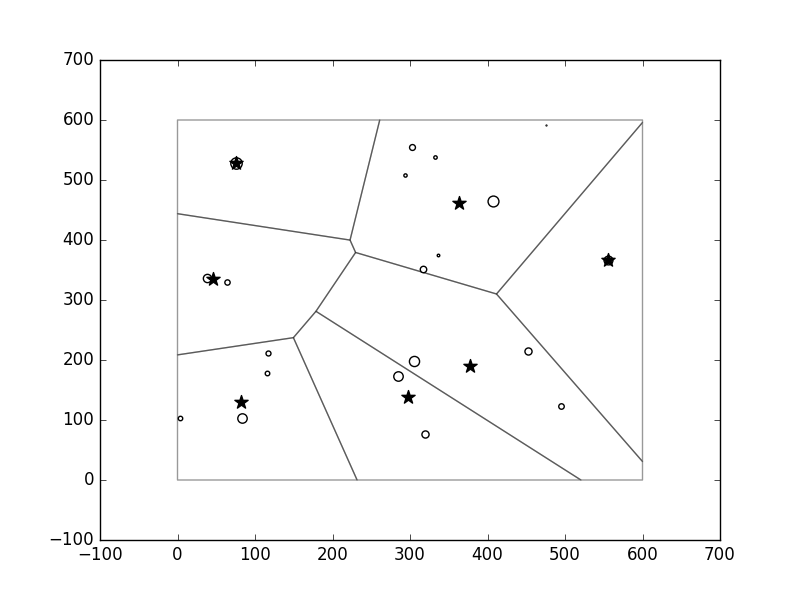
\includegraphics[width=\textwidth]{Images/1merge1.png}
  \caption{Simple re-centred Voronoi before merge.}
  \label{fig:1merge1}
\end{subfigure}
\hfill
\begin{subfigure}[b]{0.5\textwidth}
  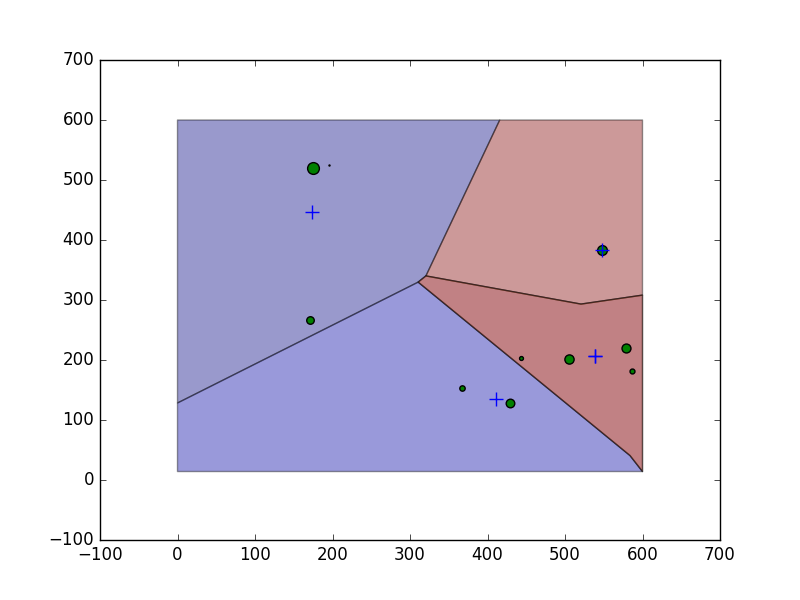
\includegraphics[width=\textwidth]{Images/1merge2.png}
  \caption{Simple re-centred Voronoi after single merge.}
  \label{fig:1merge2}
\end{subfigure}
\caption{Single merge.}
\label{fig:1merge}
\end{figure}
Figure \ref{fig:1merge} shows the effects of a single merge. As shown, the weighted distance between the merged centres is less than those of any other neighbouring centre pairs.
\begin{figure}[H]
\begin{subfigure}[b]{0.5\textwidth}
  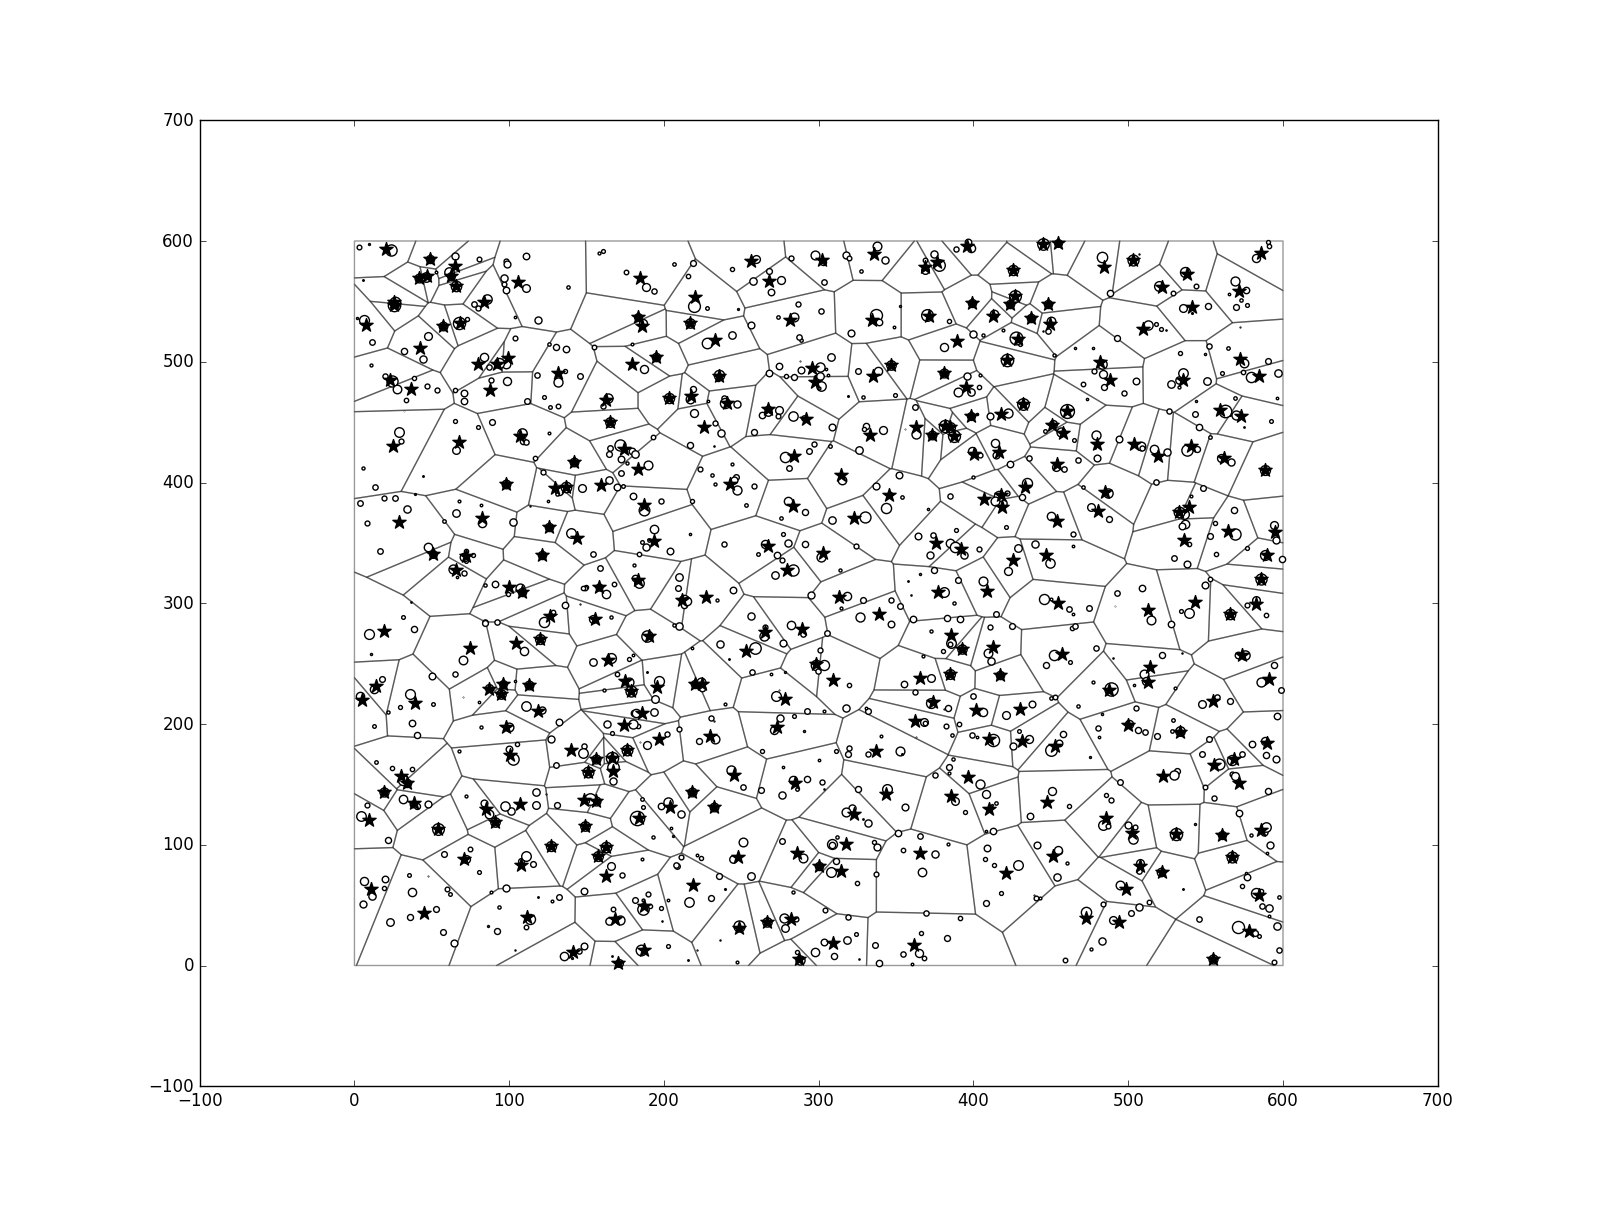
\includegraphics[width=\textwidth]{Images/merge1.png}
  \caption{Re-centred Voronoi before merge.}
  \label{fig:merge1}
\end{subfigure}
\hfill
\begin{subfigure}[b]{0.5\textwidth}
  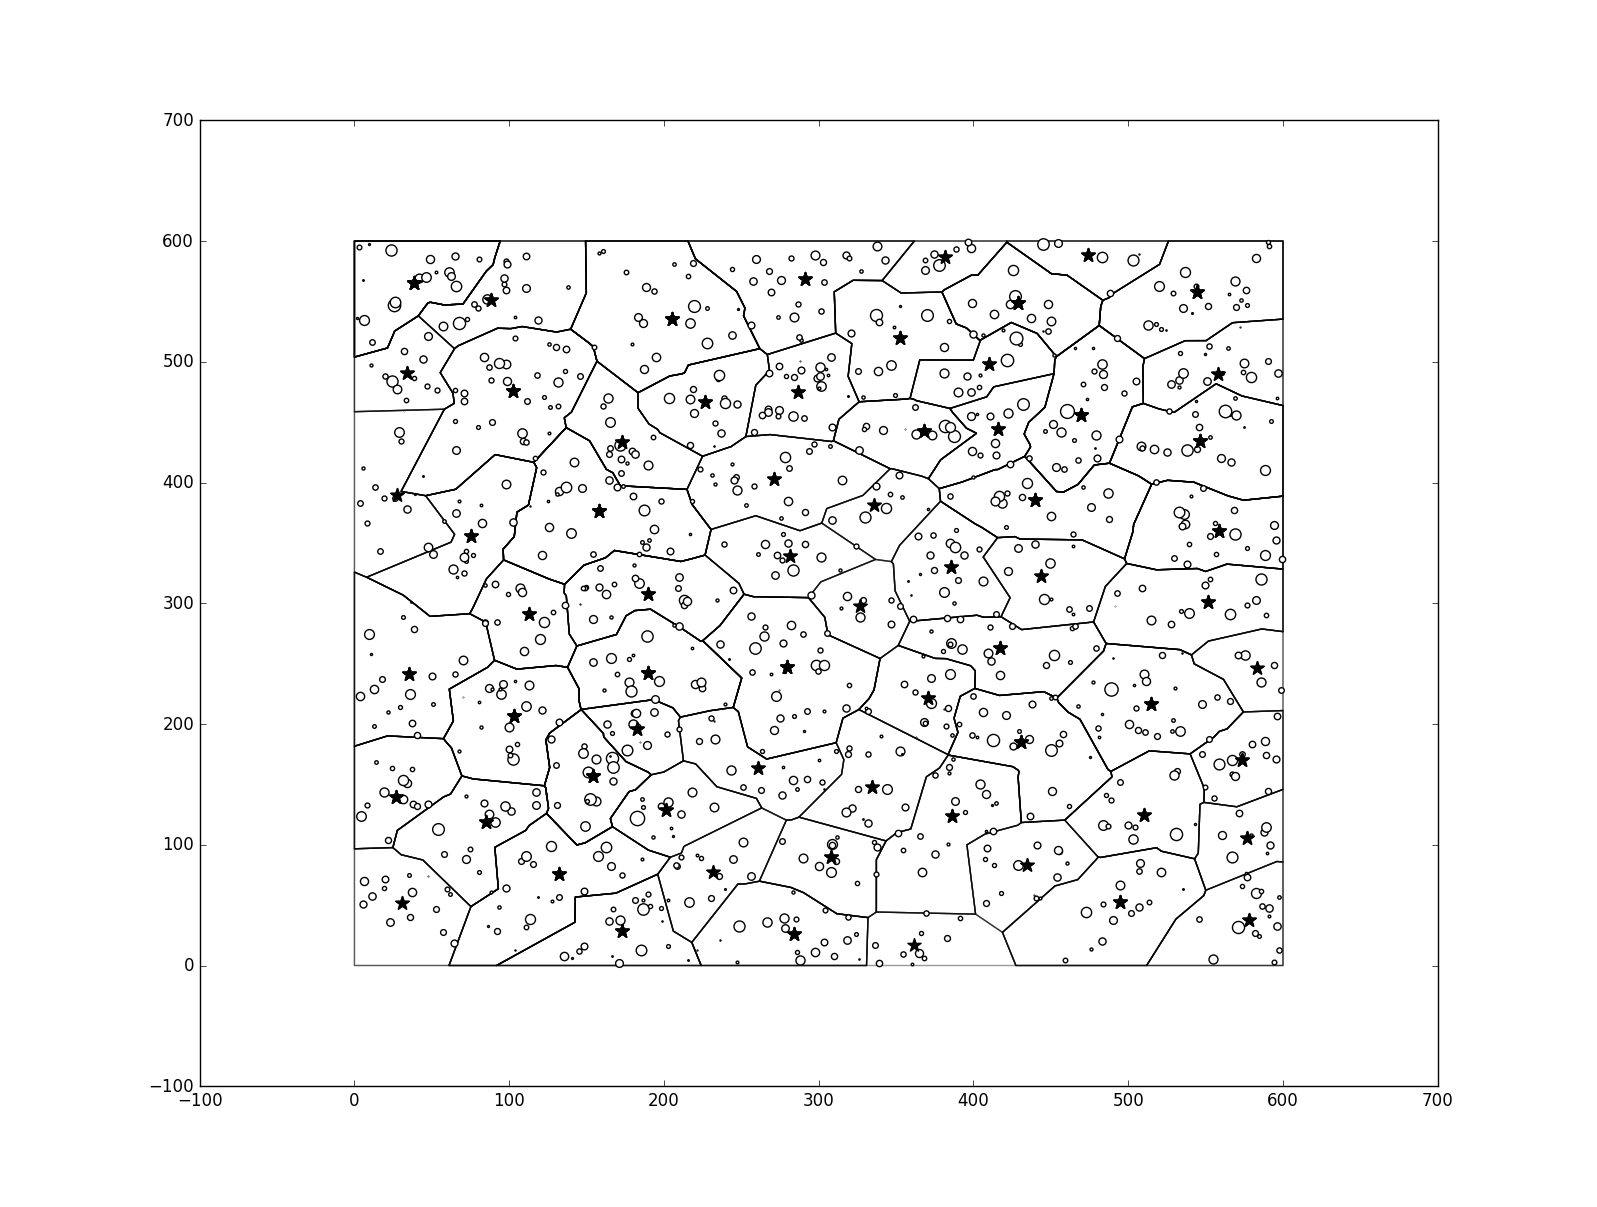
\includegraphics[width=\textwidth]{Images/merge2.png}
  \caption{Re-centred Voronoi after merge.}
  \label{fig:merge2}
\end{subfigure}
\caption{Completed merge.}
\label{fig:merge}
\end{figure}
Figure \ref{fig:merge} shows a Voronoi Tessellation and its completed merged structure, it shows larger, more centralised cell structures.